\documentclass[tikz]{standalone}

\usepackage{tikz}
\usetikzlibrary{automata}

\begin{document}

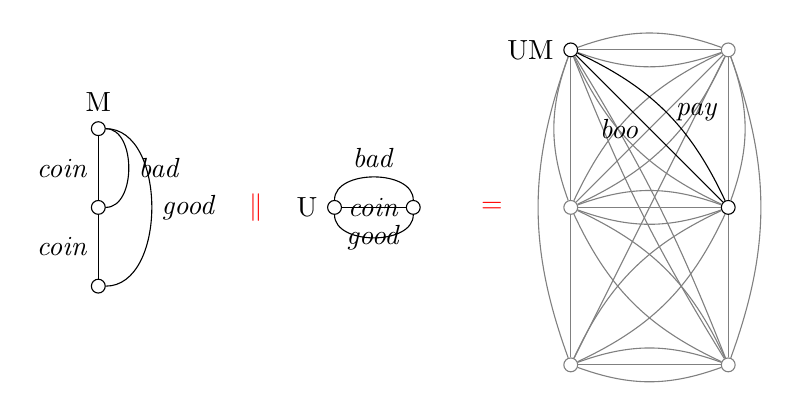
\begin{tikzpicture}
    \tikzstyle{every state}=[
        draw,
        shape=circle,
        inner sep=1pt,
        minimum size=5pt,
        final/.style={double,minimum size=6pt},
        initial text=]
    
    [->,auto]
    \renewcommand{\a}[1]{\textit{#1}}
    \begin{scope}[yshift=1cm]
    \node[state] [label=above:M] (n0) {};
    \node[state] [below of=n0] (n1) {};
    \node[state] [below of=n1] (n2) {};
    \path (n0) edge[left] node{\a{coin}} (n1)
            (n1) edge[left] node{\a{coin}} (n2)
            (n1) edge[bend right=90] node[right]{\a{bad}} (n0)
            (n2) edge[bend right=90] node[right]{\a{good}} (n0);
    \end{scope}
    \begin{scope}[xshift=3cm]
    \node[state] [label=left:U] (n0) {};
    \node[left of=n0] {\color{red}$\|$};
    \node[state] [right of=n0] (n1) {};
    \path (n0) edge node{\a{coin}} (n1)
            (n1) edge[bend left=90] node{\a{good}} (n0)
            (n1) edge[bend right=90] node[above]{\a{bad}} (n0);
    \end{scope}
    \begin{scope}[hide/.style={draw=gray},node distance=2cm,xshift=6cm,yshift=2cm]
    \node[state] [label=left:UM] (n00) {};  \node[state] [right of=n00,hide] (n10) {};
    \node[state,hide] [below of=n00]    (n01) {};  \node[state] [right of=n01] (n11) {};
    \node[state,hide] [below of=n01]    (n02) {};  \node[state] [right of=n02,hide] (n12) {};
    \node[left of=n01,node distance=1cm] {\color{red}$=$};
    \path (n00) edge[hide] (n10)
            (n10) edge[hide,bend left=20] (n00)
            (n10) edge[hide,bend right=20] (n00)
            (n01) edge[hide] (n11)
            (n11) edge[hide,bend left=20] (n01)
            (n11) edge[hide,bend right=20] (n01)
            (n02) edge[hide] (n12)
            (n12) edge[hide,bend left=20] (n02)
            (n12) edge[hide,bend right=20] (n02)
            (n00) edge[hide] (n01)
            (n01) edge[hide,bend left=20] (n00)
            (n01) edge[hide] (n02)
            (n02) edge[hide,bend left=20] (n00)
            (n10) edge[hide] (n11)
            (n11) edge[hide,bend right=20] (n10)
            (n11) edge[hide] (n12)
            (n12) edge[hide,bend right=20] (n10)
            (n01) edge[hide, bend left=20] (n12)
            (n12) edge[hide, bend left=20] (n01)
            (n10) edge[hide, bend left=20] (n01)
            (n10) edge[hide, bend right=20] (n01)
            (n01) edge[hide] (n10)
            (n11) edge[hide, bend left=20] (n02)
            (n11) edge[hide, bend right=20] (n02)
            (n12) edge[hide, bend left=5] (n00)
            (n12) edge[hide, bend right=5] (n00)
            (n02) edge[hide] (n10)
            (n00) edge[hide, bend right=20] (n11)
            (n00) edge[bend left=20] node[right]{\a{pay}} (n11)
            (n11) edge node[left]{\a{boo}} (n00);
    \end{scope}
\end{tikzpicture}
\end{document}